\section{Intensity Interferometry (II) with IACT arrays}
R. Hanbury Brown and Robert Q. Twiss (HBT) carried out the first experiments demonstrating the feasibility of measuring the angular diameters of stars using Intensity Interferometry (II) in optical wavelengths \citep{HBT56}. Subsequently, they pioneered the theoretical framework of II and conducted laboratory experiments \citep{brown1957interferometry,brown1958interferometry}, further establishing II as an alternative method to the already established Michelson Interferometry for stellar measurements. Furthermore, HBT installed the Narrabri Stellar Intensity Interferometer during the 1960s–70s and used it to measure the angular diameters of bright stars in the spectral range $\mathrm{O5f}\ -\ \mathrm{F8}$ using visible wavelength signals \citep{brown1974intensity}. However, the speed and sensitivity of electronics available in the 1970s were not sufficient for more extensive and large-scale II measurement projects.

In the early decades of the current century, proposals emerged to utilize Imaging Atmospheric Cherenkov Telescope (IACT) facilities for conducting Stellar Intensity Interferometry (SII) observations \citep{LeBohec2006, nunez2010stellar, nunez2012high, Dravins2013}. It was suggested that such observations could be carried out during bright, moonlit nights when $\gamma$-ray observations based on upper atmospheric Cherenkov showers were not feasible. This approach had the potential to enhance the scientific output of existing facilities such as VERITAS, MAGIC, and HESS. Subsequent SII observations at these facilities, providing proof of concept, have been published \citep{abeysekara2020demonstration, Abe2024MAGIC, Zmija2023}.

The remainder of this section presents a brief conceptual overview of how an array of Cherenkov telescopes is used to perform II observations and derive the Signal-to-Noise Ratio (SNR) from these measurements.

\subsection{The signal for II}\label{sec:signal}
As a simple example, let us consider a pair of IACTs pointed at a star. Suppose the two telescopes simultaneously measure the intensity of radiation $I_1(t)$ and $I_2(t)$, respectively. The signals from these detectors are cross-correlated and averaged over time, yielding the second order ($n=2$) correlation of these intensities as \citep{acciari2020optical, dravins2013optical}
\begin{equation}
	g^{(2)}= \frac{\left\langle I_1(t) \cdot I_2(t + \tau) \right\rangle}{\langle I_1(t) \rangle \cdot \langle I_2(t) \rangle} 
	\label{eqn:HBT}
\end{equation}
where $\tau$ is the time delay between the telescopes. For spatially coherent and randomly polarized light, eq.(\ref{eqn:HBT}) reduces to the Siegert relation \citep{acciari2020optical}.
\begin{equation}
	g^{(2)} = 1 + \frac{\Delta f}{\Delta \nu} \abs{V_{12}}^2
	\label{eqn:HBT2}
\end{equation}
where $\Delta f$ is the electronic bandwidth of the photon detectors (which measure the intensities and typically operate in the range $\sim 100 {\mathrm {MHz}}$) and $\Delta {\mathrm {\nu}}$ is the optical bandwidth of the radiation over which the intensities are measured.\footnote{Typically, filters with bandwidths in the range $\Delta \lambda \sim 20,\mathrm{nm} - 50,\mathrm{nm}$, corresponding to $\Delta \nu \sim 10^{15}$ Hz, are used.} In eq.(\ref{eqn:HBT2}), $V_{12}$, referred to as the complex visibility function, is the Fourier transform of the source brightness distribution and is given by
\begin{equation}
 V_{12} = 2 \frac{J_1(2 \pi d \theta)}{(2 \pi d \theta)}
\label{eqn:absvisib}
\end{equation}
where $\theta$ is the angular diameter of the star and $d$ is the radial coordinate in the conventional interferometric $(u , v) = (x/\lambda, y/\lambda)$ plane, with $\lambda$ representing the optical wavelength of the filter used for observation. It is evident from eqn(\ref{eqn:absvisib}) that $V_{12}$ contains information about the star's angular diameter. However, the phase information is lost since we measure only the absolute value $\vert V_{12} \vert^2$. In observational astronomy, the correlation is often expressed in terms of the normalized contrast, given by:
\begin{equation}
	c = \frac{\left\langle \left( I_1(t) - \left\langle I_1 \right\rangle \right) \cdot \left( I_2(t + \tau) - \left\langle I_2 \right\rangle \right) \right\rangle}{\langle I_1(t) \rangle \cdot \langle I_2(t) \rangle} = g^{(2)} - 1
\end{equation}
where, $\left\langle I_1 \right\rangle$ and $\left\langle I_2 \right\rangle$ denote the mean intensities from the two telescopes. Therefore, the signal measured by the photon detector in II, operating with an electronic bandwidth $\Delta f$ within the optical bandwidth $\Delta {\mathrm {\nu}}$ of the observational radiation, is
\begin{equation}
	c = g^{(2)} - 1 = \frac{\Delta f}{\Delta \nu} \abs{V_{12}}^2
	\label{eq:signal}
\end{equation}
$\abs{V_{12}}^2$ is a function of baseline $d = \sqrt{u^2 + v^2}$ on observational plane. Consequently, the strength of the signal is enhanced by employing a large number of baselines.

\subsection{The Signal-to-Noise Ratio for II}
\begin{figure}
	\centering
	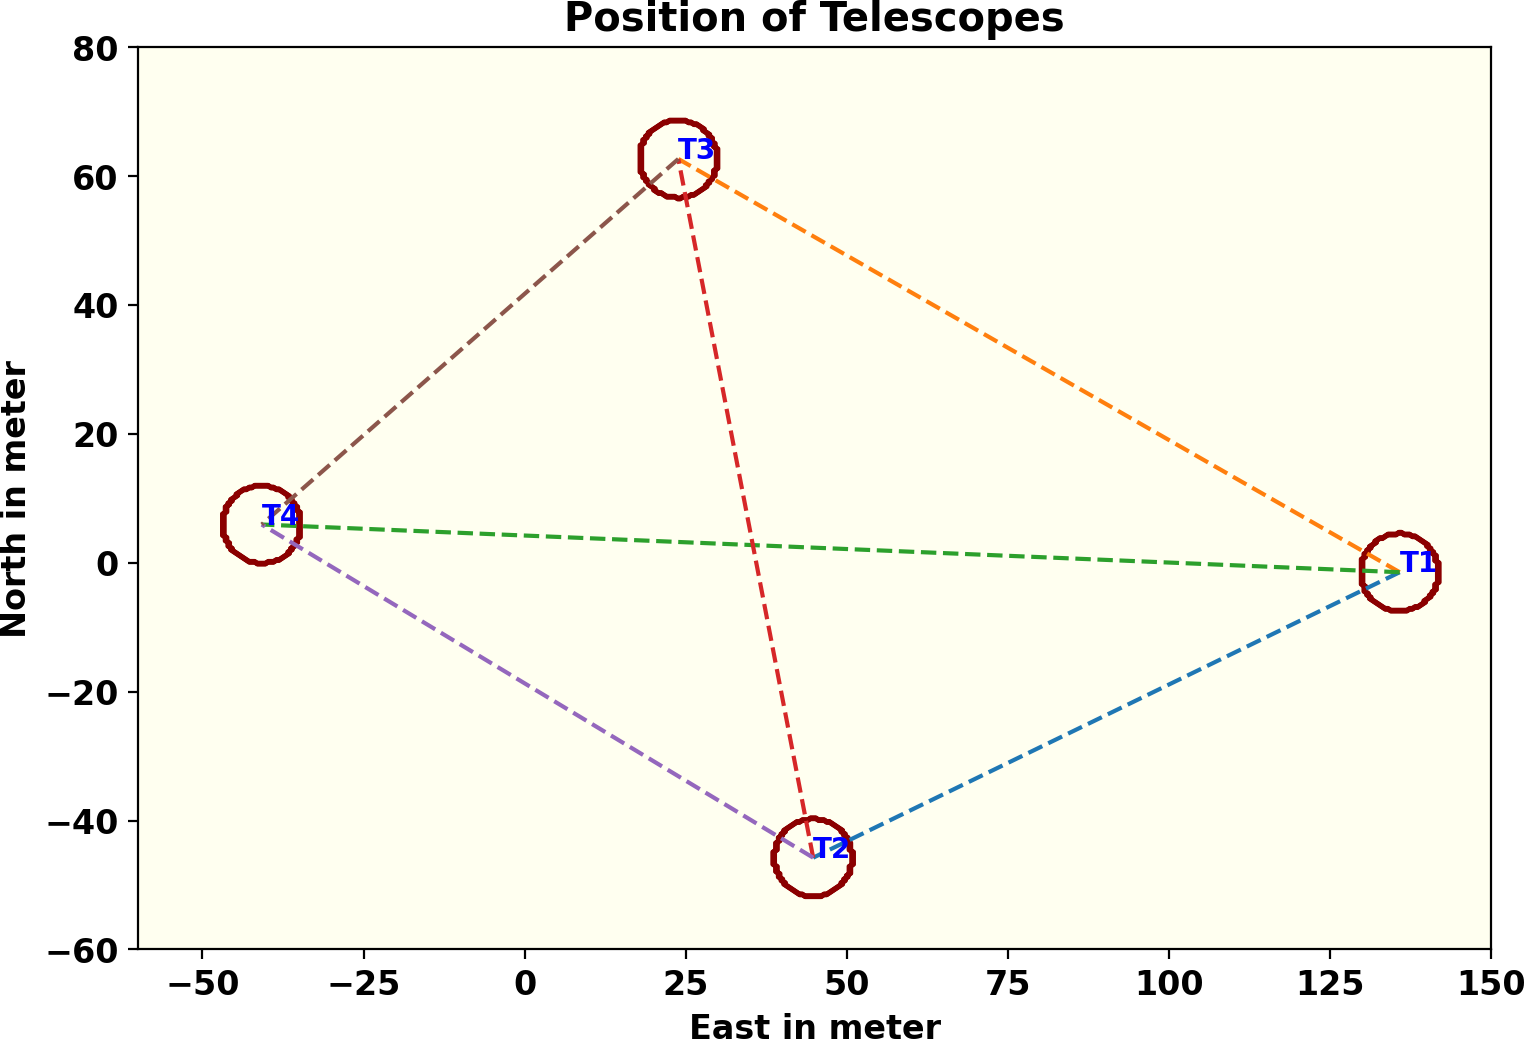
\includegraphics[width=\linewidth]{fig/telescope.png}
	\caption{The telescope configuration with similar properties each used to simulate the signal for II.}
	\label{fig:teles}
\end{figure}
\begin{figure}
	\centering
	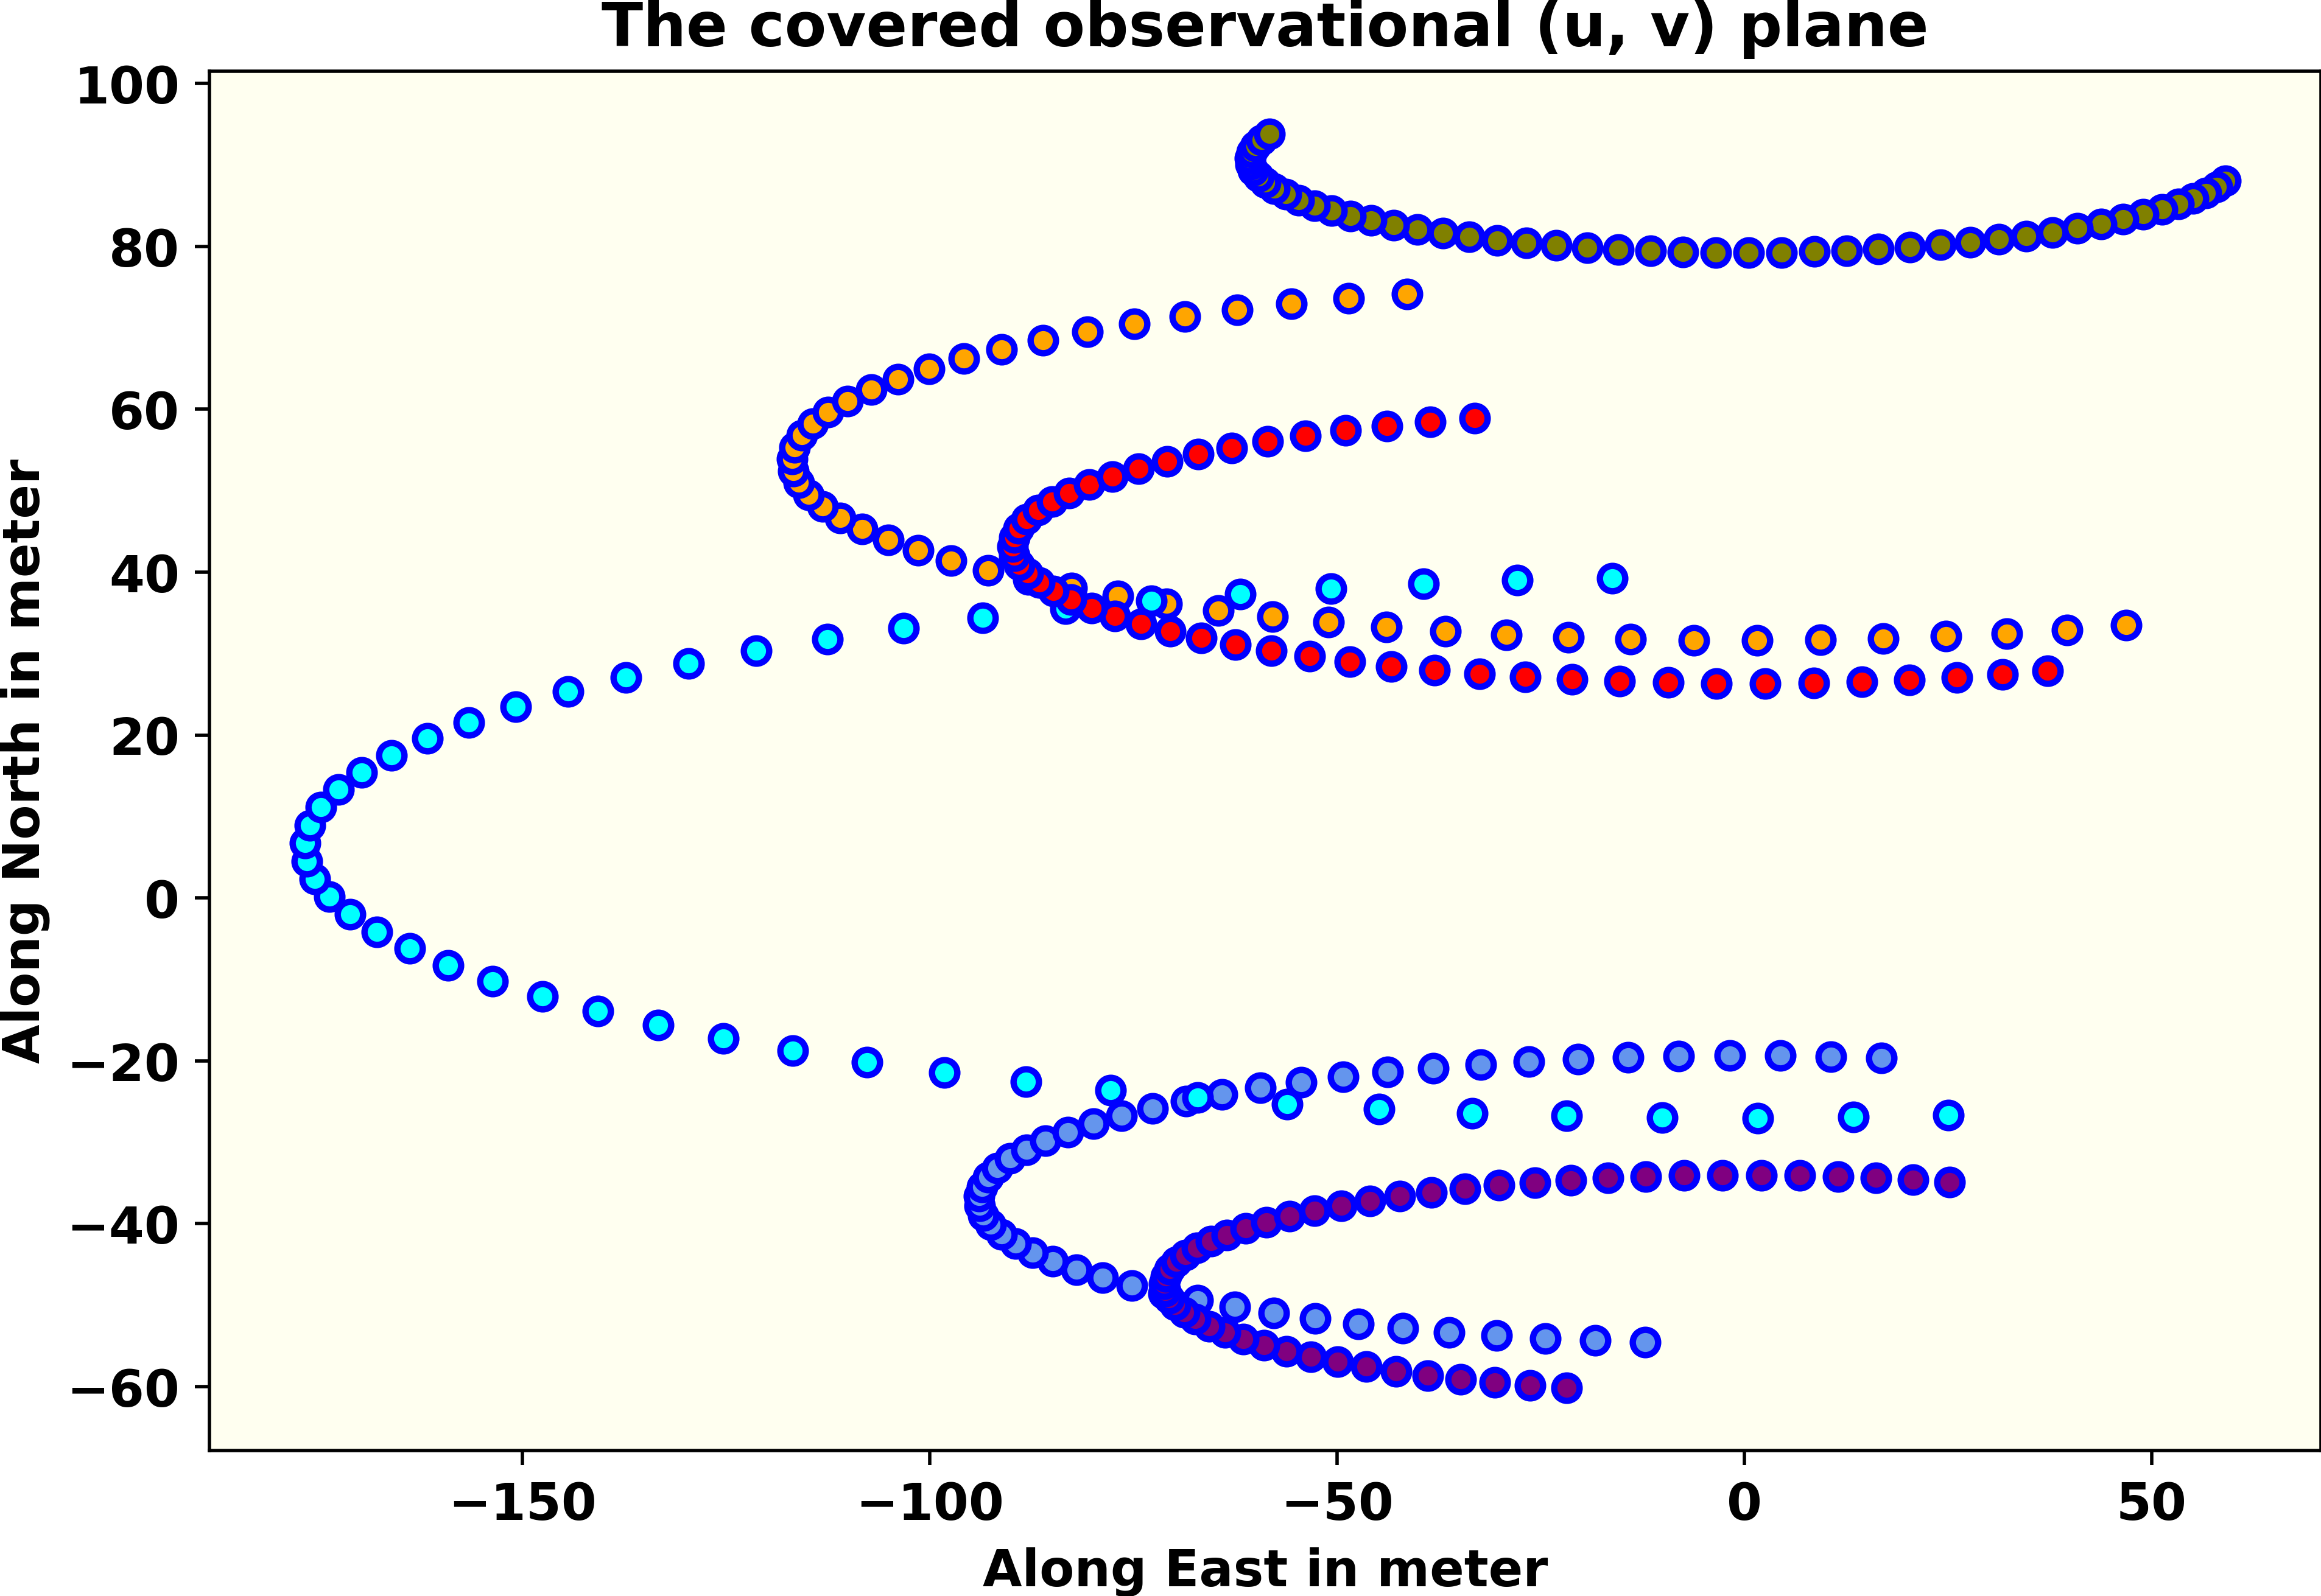
\includegraphics[width=\linewidth]{fig/baseline.png}
	\caption{The tracking of baselines with four telescopes arranged in fig.~\ref{fig:teles} for one night of observation.}
	\label{fig:base}
\end{figure}
\begin{figure}
	\centering
	\includegraphics[width=0.8\linewidth]{fig/ellipse/ellipse6018.jpg}
	\caption{This figure shows the simulated fast rotating star. The brightness is highest at the pole and there is gravitational darkening at the equator.}
	\label{fig:image}
\end{figure}
\begin{figure*}
	\centering
	\begin{subfigure}{0.5\linewidth}
		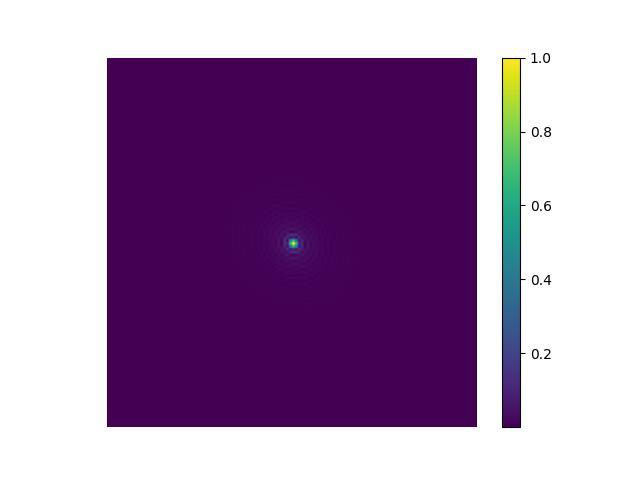
\includegraphics[width=\linewidth]{fig/ft/ft.jpg}
		\caption{The fourier transform of source.}
	\end{subfigure}\hfill
	\begin{subfigure}{0.5\linewidth}
		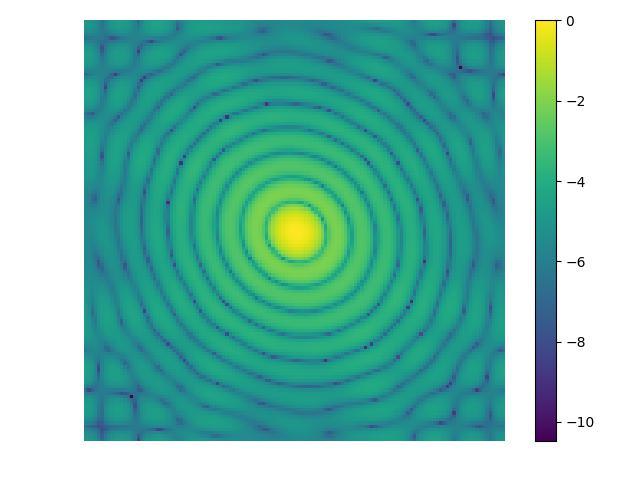
\includegraphics[width=\linewidth]{fig/ft/ft_log.jpg}
		\caption{The logarithmic fourier transform of source.}
	\end{subfigure}
	\caption{Absolute value of the two-dimensional Fast Fourier Transform of fig.~\ref{fig:image} measured by Intensity Interferometry, and observation of maximum (u, v) plane with finite number of baselines can be completed with help of earth's rotation.}
	\label{fig:ft}
\end{figure*}
\begin{figure*}
	\centering
	\begin{subfigure}{0.5\linewidth}
		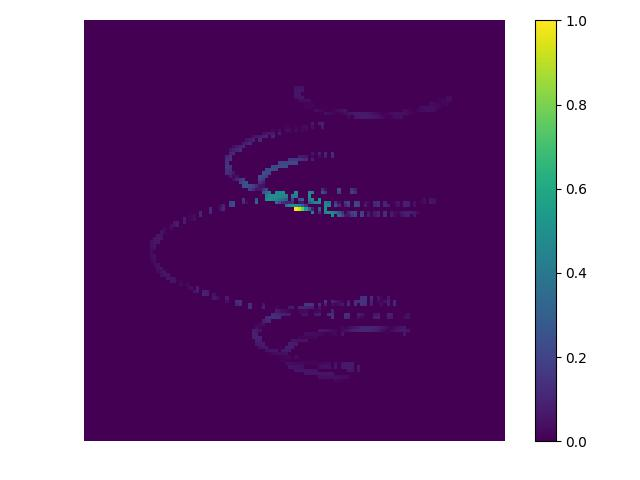
\includegraphics[width=\linewidth]{fig/ft/ft_base.jpg}
		\caption{The fourier transform with baselines.}
	\end{subfigure}\hfill
	\begin{subfigure}{0.5\linewidth}
		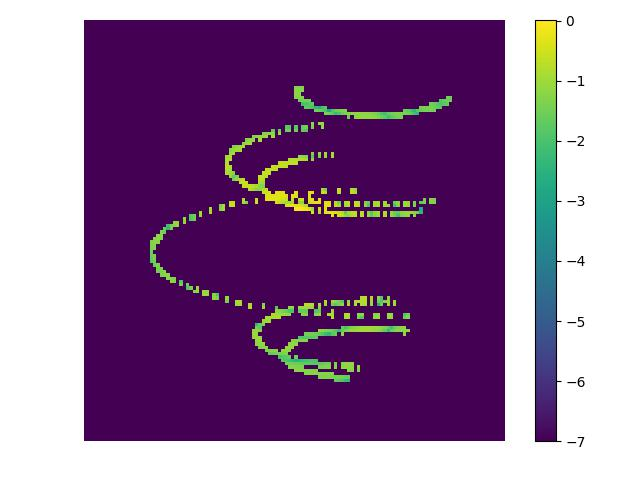
\includegraphics[width=\linewidth]{fig/ft/ft_log_base.jpg}
		\caption{The logarithmic fourier transform with baselines.}
	\end{subfigure}
	\caption{The left panel shows the absolute value of the two-dimensional Fast Fourier Transform of fig.~\ref{fig:image} measured by baselines shown in fig.~\ref{fig:teles}. The right panel shows the same on logarithmic scale}
	\label{fig:ft_base}
\end{figure*}
The primary purpose of IACTs is to study high-energy gamma rays (with energy $E\ \geq 30$ GeV) arriving from cosmic sources, entering the Earth's atmosphere, and initiating Cherenkov showers in the upper atmosphere due to multiple scattering. These telescopes feature an array of mirrors that focus light onto a set of photo-multiplier tubes (PMTs) \cite{aleksic2016major}. In the simulation model adopted here, we consider a set of four IACTs, each with similar properties. The positional configuration of these IACTs is shown in fig.~\ref{fig:teles}. The optical signal directed to a PMT is filtered using a spectral filter with a chosen mean observational wavelength $\lambda$ and corresponding bandpass $\Delta \lambda$. The use of filters not only reduces background noise but also improves the signal quality and the efficiency of the PMTs. Filtering background skylight becomes even more significant in II observations, as these are carried out during full moon nights. It is important to note that the light from the stellar source is focused on the PMT during II observations.

The significance of the signal can be expressed in terms of the signal-to-noise ratio (SNR), which depends on many factors. However, most importantly, it does not depend on the optical bandwidth $\Delta {\mathrm {\nu}}$ of the radiation for a two-telescope correlation. The explanation for the independence of the SNR from $\Delta {\mathrm {\nu}}$ is provided at the end of subsection 4.1 of \cite{10.1093/mnras/stab2391}. 
\begin{equation}
	SNR = A \cdot \alpha \cdot q \cdot n \cdot F^{-1} \cdot \sigma \cdot \sqrt{\frac{T \Delta f}{2}} \cdot \abs{V_{12}}^{2}
	\label{eq:SNR}
\end{equation}
Here, $A$ is the total mirror area, $\alpha$ is the quantum efficiency of the PMTs, $q$ is the quantum efficiency of the remaining optics, and $n$ is the differential photon flux from the source. The excess noise factor of the PMTs is represented by $F$, $T$ denotes the observation time, and $\sigma$ is the normalized spectral distribution of the light (including filters) \cite{acciari2020optical}. The signal (S) and noise (N) can be understood using eqns.\ref{eq:signal} and \ref{eq:SNR} as:
\begin{equation}
	S = \frac{\Delta f}{\Delta \nu} \abs{V_{12}}^2
\end{equation}
and
\begin{equation}
	N = (A \cdot \alpha \cdot q \cdot n \cdot F \cdot \sigma \cdot \Delta \nu)^{-1}\sqrt{\frac{2 \Delta f}{T}}.
\end{equation}
While most of the parameters can be optimized with hardware, the only way to achieve a better SNR with fixed telescopes is to increase the observation time $T$.

\subsection{Baseline considerations}
The measurement of the size of stellar objects via absolute visibility depends on the distance between the telescopes, known as the baseline $d$.
\begin{equation}
	V_{12}(d) = \frac{c(d)}{c(0)}
	\label{eq:angular_size_meas}
\end{equation}
For achieving a good SNR with a given telescope configuration, covering the largest possible observational plane is always desirable \citep{acciari2020optical, abeysekara2020demonstration}. If the source is at the zenith, the coordinates in the Fourier plane ($u,v$) are given by:
\begin{equation}
	(u,v) = \frac{1}{\lambda} (d_E, d_N)
\end{equation}
where $d_E$ and $d_N$ are the baselines expressed in east and north coordinates. However, not all sources are at the zenith, and the telescopes are stationary and may also have different relative altitudes $d_A$ depending on the available terrain. Therefore, the Earth's rotation must be taken into account to cover the maximum observational plane using rotated baselines. For a given stellar source with declination $\delta$ and hour-angle $h$, as observed by telescopes at latitude $l$, equation (\ref{eq:baseline_rot}) provides the rotated baselines for a given pair of telescopes \citep{dravins2013optical, saha2020theory}.
\begin{equation}
\begin{pmatrix} u\\ v\\ w\\ \end{pmatrix} = R_x(\delta) \cdot R_y(h) \cdot R_x(-l) \begin{pmatrix} d_E \\ d_N \\ d_A \\ \end{pmatrix}
	\label{eq:baseline_rot}
\end{equation}

The three rotation matrices $R_i$ correspond to the fundamental representation of the SO(3) group \cite{saha2020theory}. Fig.\ref{fig:base} shows the track of six baselines generated from the telescopes (fig.\ref{fig:teles}) due to Earth's rotation. Since every pair of telescopes traces an ellipse in the Fourier plane, the total number of ellipses scales as follows: 
\begin{equation}
	\label{eq:N_telescopes}
	\mathcal{N} = \frac{N_T \cdot (N_T -1)}{2}
\end{equation}
where $N_T$ is the number of telescopes considered.
As the number of baselines increases non-linearly, Intensity Interferometry (II) benefits greatly from a large number of telescopes. The planned Cherenkov Telescope Array (CTA) will cover the maximum observational plane and provide insight into stellar objects with optical wavelengths in the future.

\subsection{A Fast Rotating Star: The Object in Our Instance}
In our work presented here, we simulate a single fast-rotating star to test image reconstruction using a GAN. Fast rotation causes stars to adopt an oblate shape, flattening at the poles and bulging at the equator due to the stronger centrifugal force \cite{von1924radiative, 1999A&A...347..185M}. Fig.~\ref{fig:image} shows one of the simulations of such a fast-rotating star, with brightness distributed across its surface. The brightness is highest at the poles and lowest at the equator, a phenomenon known as gravity darkening \cite{lucy1967gravity}. This effect was first observed through interferometric and spectroscopic data from the CHARA Array for the fast-rotating star Regulus \cite{mcalister2005first}. Fast-rotating stars are crucial for understanding various astrophysical processes, including stellar evolution, internal structure, and dynamical behavior over time.

Intensity Interferometry measures (or counts) the photons arriving at the telescopes from the stellar object. The correlation of these photon arrivals at the telescopes yields the squared visibility (explained in subsection.\ref{sec:signal}). According to Van Cittert Zernike's theorem, this signal is the Fourier transform of the brightness distribution in the sky. Fig.\ref{fig:ft} represents the Fourier Transform of the source shown in fig.\ref{fig:image} using II, displayed on both linear and logarithmic scales. In order to observe a real stellar source, however, one would need to receive photons from every point on the surface of the source, which would require an infinite number of baselines observing the source over a sufficiently long duration—an obviously unfeasible demand. In practice, we have a finite number of baselines corresponding to the finite number $N_T$ of telescopes at our disposal and a limited observation schedule. Therefore, as a pilot, we have simulated the II observation of a sky source over one night's duration. Using this finite amount of signal from one night's observation, we have trained a Generative Adversarial Network (GAN) to construct the image of the source.

